\section{Технологический раздел}
В технологическом разделе будет рассмотрен подход к реализации программы, представлен внешний вид интерфейса. Также будут перечислен набор тестовых данных для некоторых функций программы.

\subsection{Выбор используемых технологий}
Далее будут представлены используемые технологии, и обоснован их выбор.

\subsubsection{Выбор ЯП}
Основные два требования, которые предъявляются к языку программирования в рамках поставленной задачи:
\begin{enumerate}
	\item высокая производительность;
	\item поддержка ООП;
	\item наличие средств профилирования;
	\item существование библиотек для замера времени.
\end{enumerate}

Всем перечисленым выше требованиям отвечает язык <<С++>> стандарта 20-го года \cite{bib:cpp_oop}.

\subsubsection{Выбор фреймворка}
Одно из ограничений курсовой работы --- запрет на использование уже существующих решений для отрисовки трёхмерной сцены. Так как алгоритм будет разрабатываться самостоятельно, производительность не является основным критерием для выбора фреймворка. От него требуется возможность отрисовать на экране сетку пикселей. Также фреймворк должен предоставлять средства разработки графического интерфейса.

Всем вышеперечисленым требованиям удовлетворяет пакет программ <<Qt>>, он и будет использоваться для создания интерфейса и отрисовки сетки пикселей на экране \cite{bib:qt_framework}.

\subsubsection{Выбор среды программирования}
Qt creator --- кроссплатформенная среда разработки, разработана специально для работы с фреймворком Qt. Несмотря на это, в качестве среды программирования (далее IDE) был использован Microsoft Visual Studio 2020. Таков выбор объясняется тем, что данная IDE предоставляет \cite{bib:visual_studio}:

\begin{itemize}
	\item систему решений, позволяющих разделять программуна множество связанных между собой проектов;
	\item средства профилирования, графически выделяющие строчки кода, занимающие большую долю процессорного времени;
	\item средства упрощённой работы с git.
\end{itemize}

Таким образом, в качестве IDE используется Microsoft Visual Studio 2020.

\subsection{Интерфейс пользователя}
Интерфейс программы представлен на рисунке \ref{fig:interface}.

\begin{figure}[ht]
	\centering
	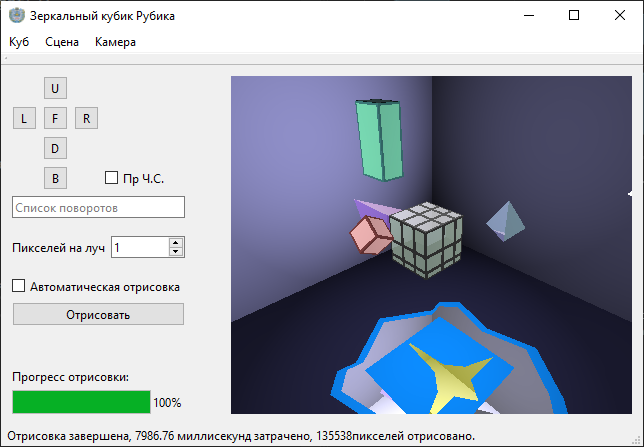
\includegraphics[width=0.9\linewidth]{interface}
	\caption{Интерфейс программы}
	\label{fig:interface}
\end{figure}

Справа находится окно просмотра, в котором отображается сцена после отрисовки. Основные элементы управления программой находятся слева.

\subsubsection{Кнопки, флаги, поля}
Кнопки U, L, F, R, D, B выполняют соответствующий поворот зеркального кубика Рубика, по отношению к изначальной позиции камеры. Флаг Пр. Ч. С. переключает кнопки U, L, F, R, D, B на U', L', F', R', D', B', функция которых меняется в соответствии с названием.

Список поворотов --- поле только для чтения, в которое записывается каждый совершённый поворот.

Пикселей на луч --- числовое поле, позволяющее установить габариты квадрата из пикселей, для которого будет пущен луч. Например, при значении 3, на каждый луч будет приходиться $3\times 3$ пикселей.

Автоматическая отрисовка --- флаг, при включении которого любое действие меняющее сцену или область отрисовки будет инициировать автоматическую перерисовку.

Отрисовать --- кнопка, инициирующая рендер сцены.

\subsubsection{Меню}
Меню Куб предоставляет действия:
\begin{enumerate}
	\item <<Отменить поворот>> --- переводит куб в состояние, в котором он был до последней операции поворота грани;
	\item <<В исходное состояние>> --- переводит куб с состояние, в котором он был при запуске программы.
\end{enumerate}

Меню <<Сцена>> предоставляет действие <<Простая отрисовка>>. Переключает программу между режимами отрисовки сцены с использованием алгоритмов трассировки лучей и проецирования каркасной модели без удаления невидимых граней.

Меню <<Камера>> предоставляею опцию <<В исходное состояние>>, которая возвращает камеру на позицию, где она была в момент запуска программы.

Кроме того, в меню камера содержится подменю <<Повернуть...>> в котором перечислены 4 действия, смещающие камеру:
\begin{enumerate}
	\item <<Влево>>;
	\item <<Вправо>>;
	\item <<Вверх>>;
	\item <<Вниз>>.
\end{enumerate}

\subsection{Тестирование}
Для тестирования методов, работающих с математическими структурами, используется система автоматического тестирования Microsoft Visual Studio CPP Unit Test Framework. На листинге \ref{lst:testcode} представлен пример тестирующего класса.

TEST\_CLASS --- группа тестов, соответствующая классу программы; TEST\_METHOD --- метод, в котором прописаны тесты для соответствующего тестируемого метода класса. Для прогонки тестов используется окно <<Test Explorer>>. Его внешний вид представлен на рис \ref{fig:test_explorer}.

\begin{figure}[ht]
	\centering
	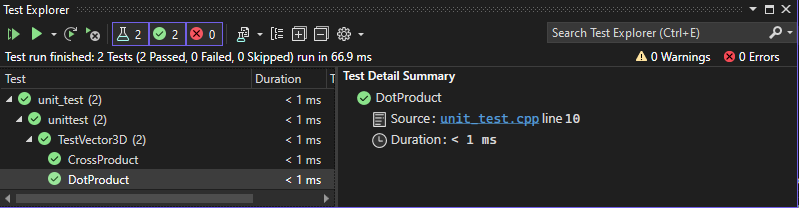
\includegraphics[width=1\linewidth]{img/test_explorer}
	\caption{Окно Test Explorer}
	\label{fig:test_explorer}
\end{figure}
\clearpage

\begin{lstlisting}[caption={Класс, реализующий тестирование методов для работы с трёхмерным вектором},label={lst:testcode},language=c++]
#include "pch.h"
#include "CppUnitTest.h"

using namespace Microsoft::VisualStudio::CppUnitTestFramework;

namespace unittest {	
	TEST_CLASS(TestVector3D) {
		public:
		TEST_METHOD(DotProduct) {
			Assert::AreEqual(Vector3D(4,-6,2)*Vector3D(2,3,3),-4.);
			Assert::AreEqual(Vector3D(2,3,3)*Vector3D(4,-6,2),-4.);
			Assert::AreEqual(
			Vector3D::dot_product(Vector3D(4,-6,2),Vector3D(0,0,0)),0.);
			Assert::AreEqual(
			Vector3D::dot_product(Vector3D(2,3,3),Vector3D(4,-6,2)),0.);
		}
		TEST_METHOD(CrossProduct) {
			auto a = Vector3D(4, -6, 2);
			auto b = Vector3D(2, 3, 3);
			Vector3D cross = Vector3D::cross_product(a, b);
			Assert::AreEqual(Vector3D(-24, -8, 24).to_string(),
				cross.to_string());
			b = Vector3D(0, 0, 0);
			cross = Vector3D::cross_product(a, b);
			for (int i = 0; i < 3; i++)
			Assert::AreEqual(0., cross[i]);
		}
	};
}
\end{lstlisting}

\subsubsection{Тестовые данные}
Далее будут приведены данные, использованные для тестирования функций, работающих с основными структурами.

Структура угла (Angle):
\begin{enumerate}
	\item real Angle::to\_radians(real) --- функция, принимающая на вход значение угла в градусах, возвращающая значение угла в радианах. Тестовые данные приведены в таблице \ref{tbl:to_radians}.
	\item real Angle::to\_degrees(real) --- функция, принимающая на вход значение угла в радианах, возвращающая значение угла в градусах. Тестовые данные приведены в таблице \ref{tbl:to_radians}.
	\begin{table}[!ht]
		\centering
		\caption{Тестовые данные для функций real Angle::to\_radians(real) и real Angle::to\_degrees(real)}
		\label{tbl:to_radians}
		\begin{tabular}{|c|c|l|}
			\hline
			Угол в градусах & Угол в радианах & Класс эквивалентности \\
			\hline
			180	& $\pi$	& Половина окружности \\
			90	& $\frac{\pi}{2}$ & Четверть окружности \\
			45	& $\frac{\pi}{4}$ & Произвольный случай \\
			-90 & $-\frac{\pi}{2}$ & Отрицательный угол \\
			0	& 0 & Нулевой угол \\
			\hline
		\end{tabular}
	\end{table}
	
	\item real Angle::optimize\_degrees(real) --- функция, приводящий произвольный угол $\alpha\in\mathbb{R}$, заданный в градусах к углу $\beta\in\left[0; 360\right)$, заданному в градусах. Тестовые данные для этой функции приведены в таблице \ref{tbl:optimize_radians}
	\begin{table}[!ht]
		\centering
		\caption{Тестовые данные для функции Angle::optimize\_degrees(real)}
		\label{tbl:optimize_radians}
		\begin{tabular}{|c|c|l|}
			\hline
			Вход & Выход & Класс эквивалентности \\
			\hline
			$\frac{5\pi}{2}$ & $\frac{\pi}{2}$ & Больше окружности \\
			$-\frac{\pi}{2}$ & $\frac{3\pi}{2}$	& Отрицательный угол \\
			$\frac{\pi}{2}$ & $\frac{\pi}{2}$ & Уже нормализованный угол \\
			$0$ & $0$ & Нулевой угол\\
			$2\pi$ & $0$ & Ровно окружность\\
			\hline
		\end{tabular}
	\end{table}
	
	\item real Angle::optimize\_degrees(real) --- функция, приводящий произвольный угол $\alpha\in\mathbb{R}$, заданный в радианах к углу $\beta\in\left[0; 2\pi\right)$, заданному в радианах. Тестовые данные для этой функции приведены в таблице \ref{tbl:optimize_degrees}
	\begin{table}[!ht]
		\centering
		\caption{Тестовые данные для функции Angle::optimize\_degrees(real)}
		\label{tbl:optimize_degrees}
		\begin{tabular}{|c|c|l|}
			\hline
			Вход & Выход & Класс эквивалентности \\
			\hline
			540 & 180 & Больше окружности\\
			-90 & 270 & Отрицательный угол\\
			90 & 90 & Уже нормализованный угол\\
			0 & 0 & Нулевой угол\\
			360 & 0 & Ровно окружность\\
			\hline
		\end{tabular}
	\end{table}
\end{enumerate}

\subsubsection{Окно просмотра}
Оценка правильности полученного изображения была проведена с помощью визуального анализа. В качестве вспомогательного инструмента, была реализована функция отображения сцены в каркасном виде без удаления граней. Внешний вид окна просмотра при работе этой функции представлен на рис. \ref{fig:scenecarcass}

\begin{figure}[ht]
	\centering
	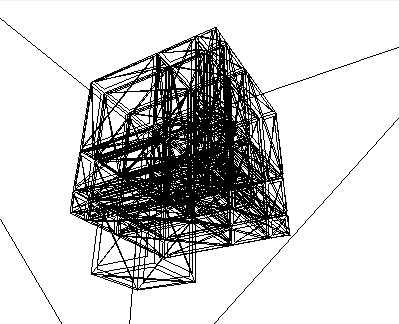
\includegraphics[width=0.7\linewidth]{img/scene_carcass}
	\caption{Окно просмотра в режиме простой отрисовки}
	\label{fig:scenecarcass}
\end{figure}

\subsection{Вывод по разделу}
В технологическом разделе представлены все использованные программные средства с обоснованием их выбора, а именно:
\begin{itemize}
	\item C++ стандарта 20-го года;
	\item Qt фреймворк;
	\item Microsoft Visual Studio 2020.
\end{itemize}

Представлены методы тестирования программы, тестовые данные и описан интерфейс пользователя.

